\chapter{Fiducial marker based visual inertial SLAM}

Results presented in this section are taken from our published work \cite{fourmy2019absolute}.

\section{Introduction}

In this work, we are interested in quantifying how accurately a humanoid robot can be localized in a structured 3D environment.
The seminal works on localization of legged robots were using leg odometry, quickly followed by contributions fusing the kinematics 
with inertial measurements~\cite{lin_hexafusion_tro06}. Evidently, odometry measurements can only lead to a drift of the localization.
Based on leg odometry, the community has extended the localization performances by improving the behavior of the inertial-kinematic 
filter~\cite{bloesch2013state,rotella2014state,flayols2017experimental}, the underlying contact 
model~\cite{bledt2018cheetah,rotella2018unsupervised}, and by augmenting the odometer with exteroceptive measurements coming from cameras or LIDAR.

%\begin{figure}[tb]
%\centering
%\includegraphics[width=0.7\linewidth]{figures/HRP2_compact_crop.jpg}
%\caption{HRP2 robot with which were conducted the experiments. The head was replaced by our visual inertial system %described in section \ref{sec:} (note that the stereo camera of the robot is not used)}
%\label{fig:HRP2}
%\end{figure}

The difficulty in fusing inertial, kinematics and exteroceptive measurements stems from the disparity in the properties of each data source.
Inertial and kinematic measurements come at high frequency (typically 100 Hz to 1 kHz) and are cheap to process, while images and laser scans 
are obtained at some few images per second and are expensive to process. 
On the other hand, inertial measurements are quickly deprecated while images and scans provide absolute information.
This implies a rigorous synchronization between the sensors with the risk of decreasing the performances of the inertial 
estimation when images and laser scans are not carefully merged. 

These difficulties explain that the first works to merge proprioceptive and exteroceptive sensors for legged localization 
have been with some staggered approach, first fusing inertial and kinematic measurements at high frequency, and then correcting 
the localization drift with absolute localization computed from camera and/or LIDAR with low bandwidth and higher delay~\cite{nobili2017heterogeneous,fallon2014drift}.

Very recently, several concurrent approaches have been proposed to merge all relevant data in a unique estimator.
Following the recent results in UAVs localization~\cite{KAESS-11-ISAM2,leutenegger_keyframe_ijrr15}, optimal estimation 
structured by a factor graph is a very nice framework to formulate the fusion.
In~\cite{hartley_graphslam_iros18}, a graph-SLAM is proposed to fuse inertial, kinematics and visual data.
Inertial measurements are considered using Forster's pre-integration factors~\cite{forster2017-TRO}.
Kinematics data are considered using a 6D factor which is also pre-integrated, but taking into account the hybrid nature 
of the contact dynamics using an event-based approach.
Visual factors are also expressed as 6D constraints obtained by visual odometry.
Results are reported on some 3-meters sequences with motion-capture ground truth.
In~\cite{wisth2019robust}, the graph-SLAM also considers inertial measurements through pre-integration, while kinematic
 measurements are pre-treated by the robot low-level system~\cite{bloesch_odo_rss13} and integrated directly as 6D factors without further consideration.
As this work is applied to a quadruped robot, obtaining this 6D information indeed requires a complex filtering in itself. 
Finally, the visual information are considered as 2D factors in the image space, obtained from feature (KLT) matching.
Impressive experimental results are demonstrated with long outdoor sequences, using a ground-truth obtained from off-line LIDAR reconstruction.

The pros and cons of these two approaches come from the choice of the factors, but the similarities are possibly more important than the differences.
Both use a plain Forster pre-integration~\cite{forster2017-TRO}. 
Using either visual odometry or feature tracking, both systems cannot natively benefit from the information brought by loop closure, and would fail 
to exploit known map information.
In both cases, the kinematic factor is straightforward to write as a 6D constraint.
Finally, both works are able to account for the very different sensor frequencies, while providing a good estimate at the higher frequency if needed.

In this work, we are looking for a solution to localize a humanoid robot indoor, with sufficient accuracy to navigate on some stairs, grasp a handrail or 
walk on a 30-cm wide beam. 
As the robot is going to come back again and again in the same environment, we would like to benefit from loop-closure information and localization with 
respect to some known landmarks. 
While our final goal is to merge in the optimal estimator the measurements coming from all the sensors of the robot, we focus here on contributions 
validating the use of visual-inertial localization and mapping on a humanoid robot navigating indoor in a 3D environment.
For the visual factor, we rely on April tags \cite{wang_april2_iros16,he_aprilslam_ar19}, while proposing a practical contribution to avoid ambiguity 
issues in the pose estimation of the tags. 
For the inertial factor, we build upon Forster pre-integration~\cite{forster2017-TRO} and propose an original and more rigorous theoretical formulation, 
by exhibiting a Lie topology that is suitable for optimal estimation. 
This formulation, although leading to very similar results for the inertial factors, would enable an easy generalization to the other high-frequency factors 
that would typically arise in the humanoid contact (leg odometry based on coders, force sensors, etc).
Both inertial and visual factors are processed in a factor graph resulting into a nonlinear maximum-likelihood optimization problem, solved with Ceres~\cite{ceres-solver}.




\section{Problem statement}
% \section{State estimation for the humanoid}

\begin{figure}
    \centering
    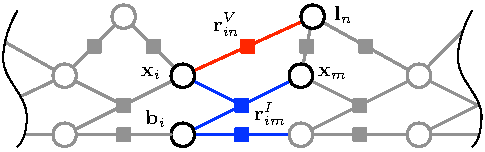
\includegraphics[scale=0.9]{figures/graph}
    \caption{A typical fraction of the factor graph, involving state blocks corresponding to keyframes $\bfx_i=(\bfp_i,\bfv_i,\bfR_i)$, biases $\bfb_i$ and landmark poses $\bfl_n$. 
    IMU factors (blue) relate consecutive keyframes and the IMU biases.
    The lower branch controls bias drift along time.
    Visual factors (red) relate landmarks with poses $(\bfp_i,\bfR_i)$.}
    \label{fig:graph}
\end{figure}

In graph-based optimization, the problem is well represented as a bipartite graph, where one type of node refers to the variables, 
and the other type called \emph{factors} represent the geometrical constraints between variables, produced by the measurements.
%
The state $\bfx$ is modeled as a multi-variate Gaussian distribution.
In the case of landmark-based visual-inertial SLAM (see \figRef{fig:graph}), $\bfx$ includes robot poses and velocities 
$\bfx_i=(\bfp_i,\bfv_i,\bfR_i)$ and sensor biases $\bfb_i$, both at selected keyframes $i$ along the trajectory, and landmark poses $\bfl_n\in\SE(3)$.
Bias are considered constant between keyframes and are taken at the $i$-th keyframe.
%
In line with the recent works on the subject, we write the MAP optimization as the least-squares minimization (\figRef{fig:graph}),
%
\begin{align}\label{equ:least_squares}
    \bfx^* = \argmin_\bfx 
    \sum_i \norm{\bfr^I_i(\bfx)}_{\bfSigma^I_i}^2
    +
    \sum_j \norm{\bfr^V_j(\bfx)}_{\bfSigma^V_j}^2
    % +
    % \sum_c \norm{\bfr_c(\bfx)}_{\Sigma_c}^2
~,
\end{align}
%
with $\{\bfr^I,\bfSigma^I\}$ and $\{\bfr^V,\bfSigma^V\}$ indicating the residuals and covariances of respectively the inertial (IMU) and visual factors.
These residuals are computed differently depending on the nature of the measurements and the state blocks they relate to. 
They are described in the following two chapters.




\subsection{Related works}
Two Apriltag based visual-inertial SLAM systems have been implemented in the previous years. 
In \cite{neunert2016open}, the authors rely on a EKF in which state propagation is naturally 
handled by the IMU and each marker detection is used in an update step where the reprojection error of its 4 corners provides a 8D innovation vector. 
A closer solution to ours was very recently proposed in \cite{he2019lightweight} and is also based on graph SLAM optimization benefiting from 
Forster's IMU pre-integration from GTSAM. As explained previously, the Apriltag factor formulation is different from ours and the algorithm is tested 
on large datasets consisting only of smooth motions.


\subsection{Results}

\subsubsection{Experimental setup}
